% This file is for tex not in the paper but which I don't want to delete
% just yet in case we want it later.%
We consider a few cases, depending on how $\KL{\eta, \t}$ is evaluated.
For illustration, we consider the following simple example.

\begin{ex}\exlabel{q_normal}
%
Let $\x \in \mathbb{R}$, $\theta \in \mathbb{R}$, $p(\x \vert \theta) = \normdist{\x
\vert \theta, 1}$, and $p(\theta \vert \t) = \normdist(\theta \vert \t, 1)$.  Then
%
\begin{align*}
%
\logp(\x \vert \theta) ={}&
    -\frac{1}{2} \left(\theta^2 - 2 \theta \x \right) + \const
    & \constdesc{\theta} \\
\logp(\theta \vert \t)={}&
    -\frac{1}{2} \left(\theta^2 - 2 \theta \t \right) + \const
    & \constdesc{\theta} \Rightarrow  \\
\logp(\x \vert \theta) + \logp(\theta \vert \t)={}&
    \theta(\x - \t) - \theta^2 + \const.
    & \constdesc{\theta}.
%
\end{align*}
%
Let $\eta = (\mu, \sigma)^T$ and $\q(\theta \vert \eta) = \normdist{\theta \vert \mu,
\sigma^2}$, so that
%
\begin{align*}
%
\log \q(\theta \vert \eta) &=
    -\frac{1}{2} \sigma^{-2} (\theta - \mu)^2 -\frac{1}{2} \log \sigma^2 +
    \const.&\constdesc{\theta, \eta}
%
\end{align*}
%
\end{ex}

In the simplest case, we can evaluate $\expect{\q(\theta \vert \eta)}{ f(\theta,
\t) }$ explicitly as a funciton of $\eta$, in which case we can compute
the needed derivatives exactly.

\begin{ex}\exlabel{q_normal_exact}
%
In \exref{q_normal}, we can compute
TODO(fix this)
%
\begin{align*}
%
\expect{\q(\theta \vert \eta)}
       {-\logp(\x \vert \theta) - \logp(\theta \vert \t)} ={}&
\expect{\q(\theta \vert \eta)}{\theta(\t - \x) + \theta^2 + \const}
    %& \constdesc{\theta}
\\={}&
\mu (\x - \t) - \mu^2 - \sigma^2  + \const %& \constdesc{\eta}
%
\end{align*}
%
and
%
\begin{align*}
%
\expect{\q(\theta \vert \eta)}{\log \q(\theta \vert \eta)} ={}&
\expect{\q(\theta \vert \eta)}
       {-\frac{1}{2} \sigma^{-2} (\theta - \mu)^2 -\frac{1}{2} \log \sigma^2 +
        \const} %&\constdesc{\theta, \eta}
\\={}& \frac{1}{2} \log \sigma^2 + \const. %&\constdesc{\eta}.
%
\end{align*}
%
So
%
\begin{align*}
%
\KL{\eta, \t} ={}&
    \mu (\x - \t) - \mu^2 - \sigma^2 + \frac{1}{2} \log \sigma^2 +
    \const,
    &\constdesc{\eta}
%
\end{align*}
%
and we can directly compute
%
\begin{align*}
%
\fracat{\partial \KL{\eta, \t}}{\partial\eta}{\eta, \t} ={}&
    \left(\begin{array}{c}
    \x - \t - 2\mu\\
    -2\sigma + \sigma^{-1}
    \end{array}\right)\\
\fracat{\partial^2 \KL{\eta, \t}}{\partial\eta \partial \eta^T}{\eta, \t} ={}&
    \left(\begin{array}{cc}
    -2          &           0\\
    0           &           -2 - \sigma^{-2}
    \end{array}\right)\\
%
\end{align*}
%


%
\end{ex}






Observe that
%
\begin{align*}
%
\log \pstick(\nuk \vert \phi) ={}&
    \log \pb(\nuk) + \phi(\nuk) + \const
    & \constdesc{\nuk} \Rightarrow\\
\KL{\eta, \phi} ={}&
    \KL{\eta, 0} + \sumkm \expect{\q(\nuk \vert \eta)}{\phi(\nuk)}.
%
\end{align*}
%
Let $\phiz(\cdot)$ denote the zero function.  Then, using \eqref{vb_eta_sens}
gives that the directional (Gateaux) derivative in the direction $\phi$
evaluated at $\phiz$ is given by
%
\begin{align*}
%
\fracat{d \etaopt(\phi)}{d \phi}{\phiz} ={}&
    - \hess{\zeta\zeta}^{-1}
    \evalat{
        \sumkm \frac{\partial}{\partial \eta}
            \expect{\q(\nuk \vert \eta)}{\phi(\nuk)}}
           {\etaopt(\phiz), \phiz}.
%
\end{align*}
%
Differentiating under the integral in $\expect{\q(\nuk \vert
\eta)}{\phi(\nuk)}$ gives
%
\begin{align*}
%
\evalat{
\frac{\partial}{\partial \eta}
    \expect{\q(\nuk \vert \eta)}{\phi(\nuk)}
}{\etaopt} ={}&
\expect{\q(\nuk \vert \etaoptnuk)}
       {\evalat{\frac{\partial}{\partial \etanuk}
                  \log\q(\nuk \vert \etanuk)}
                {\etaoptnuk}
        \phi(\nuk)} \\
={}&
\int_0^1
    \q(\nu \vert \etaoptnuk)
    \evalat{\frac{\partial}{\partial \etanuk}
               \log\q(\nu \vert \etanuk)}
             {\etaoptnuk}
    \phi(\nu) d\nu.
%
\end{align*}
%
Plugging in gives
%
\begin{align*}
%
\fracat{d \etaopt(\phi)}{d \phi}{\phiz} =&{}
    \int_0^1
    -\hess{\zeta\zeta}^{-1}
    \left(
        \sumkm
        \q(\nu \vert \etaoptnuk)
        \fracat{\partial \log\q(\nu \vert \etanuk)}
               {\partial \etanuk}
               {\etaoptnuk}
    \right) \phi(\nu) d\nu.
%
\end{align*}
%
Thus, the influence function for $\etaopt(\phi)$ at $\phiz$ is given by
%
\begin{align*}
%
\infl(\nu) :={}&
-\hess{\zeta\zeta}^{-1}
\left(
    \sumkm
    \q(\nu \vert \etaoptnuk)
    \fracat{\partial \log\q(\nu \vert \etanuk)}
           {\partial \etanuk}
           {\etaoptnuk}
\right) \\
\fracat{d \etaopt(\phi)}{d \phi}{\phiz} =&{}
    \int_0^1 \infl(\nu) \phi(\nu) d\nu.
%
\end{align*}
%
Analogously, for a differentiable function of interest $g(\eta)$,
the influence function is given via \eqref{vb_g_sens} to be
%
\begin{align*}
%
\inflg(\nu) :={}&
-\fracat{\partial g(\eta)}{\partial \eta^T}{\etaopt(\t_0)}
    \hess{\zeta\zeta}^{-1}
\left(
    \sumkm
    \q(\nu \vert \etaoptnuk)
    \fracat{\partial \log\q(\nu \vert \etanuk)}
           {\partial \etanuk}
           {\etaoptnuk}
\right) \\
\fracat{d g(\etaopt(\phi))}{d \phi}{\phiz} =&{}
    \int_0^1 \inflg(\nu) \phi(\nu) d\nu.
%
\end{align*}
%
The influence funciton is a convenient summary of the effect of functional prior
perturbations on a differnetiable summary statistic, as we will show below.

An additional benefit of the influence function is that it admits a closed-form
expression for the ``worst-case'' perturbation in an $\norminf{\cdot}$ ball
via Holder's inequality, since
%
\begin{align*}
%
\sup_{\phi: \norminf{\phi} \le \delta}
    \fracat{d g(\etaopt(\phi))}{d \phi}{\phiz} =&{}
\sup_{\phi: \norminf{\phi} \le \delta}
    \int_0^1 \inflg(\nu) \phi(\nu) d\nu \\
\le&{} \delta \int_0^1 \abs{\inflg(\nu) }d\nu,
%
\end{align*}
%
with equality when $\phi(\nu) = \delta \, \mathrm{sign}(\inflg(\nu))$.

In order for the supremum over a bounded set $\phi: \norminf{\phi} < \delta$
to be meaningful, a minimal requirement is that the function $\etaopt(\phi)$
be Fr{\'e}chet differentiable.





















Let us define some compact notation for the duration of the proof.
Let
%
\begin{align*}
%
\KLgrad{\eta, \phi} :={}&
    \fracat{\partial \KL{\eta, \phi}}{\partial \eta}{\eta, \phi}
\mathtxt{and}
\KLhess{\eta, \phi} :={}&
    \fracat{\partial^2 \KL{\eta, \phi}}
           {\partial \eta \partial \eta^T}{\eta, \phi}.
%
\end{align*}
%
Additionally, define $\rho(\etanuk, \phi) :={} \expect{\q(\nu \vert
\etanuk)}{\phi(\nu)}$, with
%
\begin{align*}
%
\rho_\eta(\etanuk, \phi) :={}
    % \fracat{\partial \expect{\q(\nu \vert \etanuk)}{\phi(\nu)}}
    %        {\partial \etanuk}{\etanuk} \mathand
\fracat{\partial \rho(\etanuk, \phi)}
       {\partial \etanuk}{\etanuk} \mathand
\rho_{\eta\eta}(\etanuk, \phi) :={}
   \fracat{\partial^2 \rho(\etanuk, \phi)}
          {\partial \etanuk \partial \etanuk^T}{\etanuk}.
%
\end{align*}

Observe that the estimating equation can be written as
%
\begin{align*}
%
% \KL{\eta, \phi} ={}&
%     \KL{\eta, \phiz} + \sumkm \rho(\etanuk, \phi)
%     \Rightarrow \\
%
\KLgrad{\eta, \phi} ={}&
\KLgrad{\eta, \phiz} + \sumkm \rho_\eta(\etanuk, \phi)
= 0_\etadim.
%
\end{align*}

Let us first show that $\KLgrad{\eta, \phi}$ is continuously Fr{\'e}chet
differentiable.  By \assuitemref{kl_opt_ok}{kl_diffable}, $\eta \mapsto
\KLgrad{\eta, \phiz}$ is continuously differentiable and does not depend on
$\phi$, so we need only to show that $\rho_\eta(\etanuk, \phi)$ is continuously
Fr{\'e}chet differentiable. To show this, it will suffice to show that the
partial deritatives of the maps $\eta \mapsto \rho_\eta{\eta, \phi}$ and $\phi
\mapsto \rho_\eta{\eta, \phi}$ exist and are continuous in the dual norm
$\norm{\cdot}^*$ as a function of the location $\eta, \phi$ at which the
derivatives are evaluated.

We first show that $\phi \mapsto \rho_\eta(\etanuk, \phi)$ is Fr{\'e}chet
differentiable.  To do so it


It follows from \eqref{q_sens_is_cov} that the map $\phi \mapsto
\rho_\eta(\etanuk, \phi)$ is a linear functional of $\phi$.  Applying Jensen's
inequality to the $\norm{\cdot}_2$ norm and the triangle inequality twice gives:
%
\begin{align*}
%
%\sup_{\phi: \norminf{\phi} = 1}
\norm{\rho_\eta(\etanuk, \phi)}_2 \le
    4 \expect{\q(\nu \vert \etanuk)}
             {\norm{\nabla \log \q(\nu \vert \etanuk)}_2}
              \norminf{\phi(\nu)}.
%
\end{align*}
%
It follows from ... that $\rho_\eta(\etanuk,
\phi)$ is bounded as a function of $\phi$ for all $\eta \in \ball_\eta$.
Bounded linear functionals are Fr{\'e}chet differentiable (essentially by
definition), so $\phi \mapsto \rho_\eta(\etanuk, \phi)$ is Fr{\'e}chet
differentiable.

It remains to show that the derivative is continuous.

% so the linear operator is bounded as a function of $\phi$, and a continuous
% funciton of $\eta$ by assumption.  Therefore $\phi \mapsto \fracat{\partial
% \expect{\q(\nu \vert \etanuk)} {\phi(\nu)}}{\partial \eta}{\eta}$ is
% continuously Fr{\'e}chet differentiable.
%
% Again differentiating under the integral,
% %
% \begin{align*}
% %
% \fracat{\partial^2 \expect{\q(\nu \vert \etanuk)}
%               {\phi(\nu)}}{\partial \eta \partial \eta^2}{\eta} ={}&
% \expect{\q(\nu \vert \etanuk)}
%        {\left(\nabla \log \q(\nu \vert \etanuk)
%          - \expect{\q(\nu \vert \etanuk)}
%                   {\nabla \log \q(\nu \vert \etanuk)}
%        \right)^2
%        \left( \phi(\nu) - \expect{\q(\nu \vert \etanuk)}{\phi(\nu)} \right)} +
% \\&
% \expect{\q(\nu \vert \etanuk)}{
%        \left(                            \nabla^2 \log \q(\nu \vert \etanuk)
%         - \expect{\q(\nu \vert \etanuk)}{\nabla^2 \log \q(\nu \vert \etanuk)}
%        \right)
%        \left( \phi(\nu) - \expect{\q(\nu \vert \etanuk)}{\phi(\nu)} \right)
%        }.
% %
% \end{align*}
% %
Again this is a linear operator as a function of $\phi$, which is continuous by
assumption.  Consequently the Hessian is invertible in a neighborhood.

It follows by \citet[Proposition 4.14(c)]{zeidler:2013:functional} that
$\KLgrad{\eta, \phi}$ is continuosly Fr{\'e}chet differentiable.  Furthermore,
\citet[Chapter 4 Condition 21b]{zeidler:2013:functional} holds since
$\KLhess{\etaopt(\phiz), \phiz}$ is invertible.  So we satisfy conditions (i),
(ii), and (iii) of \citet[Theorem 4.B(c)]{zeidler:2013:functional}, giving that
the function $\etaopt(\phi)$ exists.  Moreover, since $\KLgrad{\eta, \phi}$ is
continuously Fre{\'e}chet differentiable in a neighborhood of $\etaopt(\phiz),
\phiz$, by \citet[Theorem 4.B(d)]{zeidler:2013:functional}, $\etaopt(\phi)$ is
also continuously Fr{\'e}chet differentiable.

The directional derivative

% Other references: We will use the
% formulation given in \citep[Theorem 3.4.10]{krantz:2012:implicit}, for which
% we must show that... actually that doesn't give differentiability.
% The result follows then from \citet[Proposition 4.8(c)]{zeidler:2013:functional}.
% See also \citet[Corollary 1.4]{averbukh:1967:theory} and \citep[Appendix
% A]{reeds:1976:thesis}).
%
















%%%%%%%%%%%%%%%%%%%%%%%%%%%%%%%%%%%%%%%%%%%%%%%%%%%%%%%%%%%%%%%%%%%%%%%%%
%%%%%%%%%%%%%%%%%%%%%%%%%%%%%%%%%%%%%%%%%%%%%%%%%%%%%%%%%%%%%%%%%%%%%%%%%
\begin{ex}\exlabel{averbukh}
%
(\citet[Example 1.9]{averbukh:1967:theory})
%
Consider $(x_1, x_2) \in \mathbb{R}^2$ and the polar coordinates $r :=
\sqrt{x_1^2 + x_2^2}$ and $\theta := \arctan(x_2 / x_1)$.  Let $\{\pi k: k \in
\mathbb{Z} \}$ denote integer multiples of $\pi$.  Define
%
\begin{align*}
%
f(r, \theta) := \begin{cases}
\frac{r^2}{| \sin \theta |} \exp\left( -\frac{r}{|\sin \theta|}\right)
    & \textrm{when } \theta \notin \{\pi k: k \in \mathbb{Z} \} \\
0. & \textrm{when } \theta \in \{\pi k: k \in \mathbb{Z} \}
%
\end{cases}
%
\end{align*}
%
Then $f$ is continuous at $(0, 0)$ and has a directional derivative in every
direction, but is not Fr{\'e}chet differentiable.
%
\begin{proof}
%
It is easy to show that $\sup_{y \ge 0} y \exp(-y) = \exp(-1)$, which is
achieved at $y=1$. So, for any $(r_1, \theta_1)$ and $(r_2, \theta_2)$,
$\abs{f(r_1, \theta_1) - f(r_2, \theta_2)} \le \abs{r_1 - r_2} \exp(-1)$, from
which it follows that $f(r, \theta)$ is continuous at $0$.  Moreover, for any
fixed direction $\theta$, $\fracat{\partial f(r, \theta)}{\partial r}{r=0} = 0$,
so the linear approximation to $f(r, \theta)$ at $(0, 0)$ in any direction is
identically zero.  For any $r > 0$, the error in the linear approximation is
given by $\sup_{\theta} \abs{f(r, \theta) - 0} = r \exp(-1)$, which is achieved
by setting $r / |\sin \theta| = 1$.  Thus the error in the linear approximation
is of order $r$, not smaller.
%
\end{proof}
%
\end{ex}
%%%%%%%%%%%%%%%%%%%%%%%%%%%%%%%%%%%%%%%%%%%%%%%%%%%%%%%%%%%%%%%%%%%%%%%%%
%
%%%%%%%%%%%%%%%%%%%%%%%%%%%%%%%%%%%%%%%%%%%%%%%%%%%%%%%%%%%%%%%%%%%%%%%%%
%%%%%%%%%%%%%%%%%%%%%%%%%%%%%%%%%%%%%%%%%%%%%%%%%%%%%%%%%%%%%%%%%%%%%%%%%
\begin{figure}[h!]

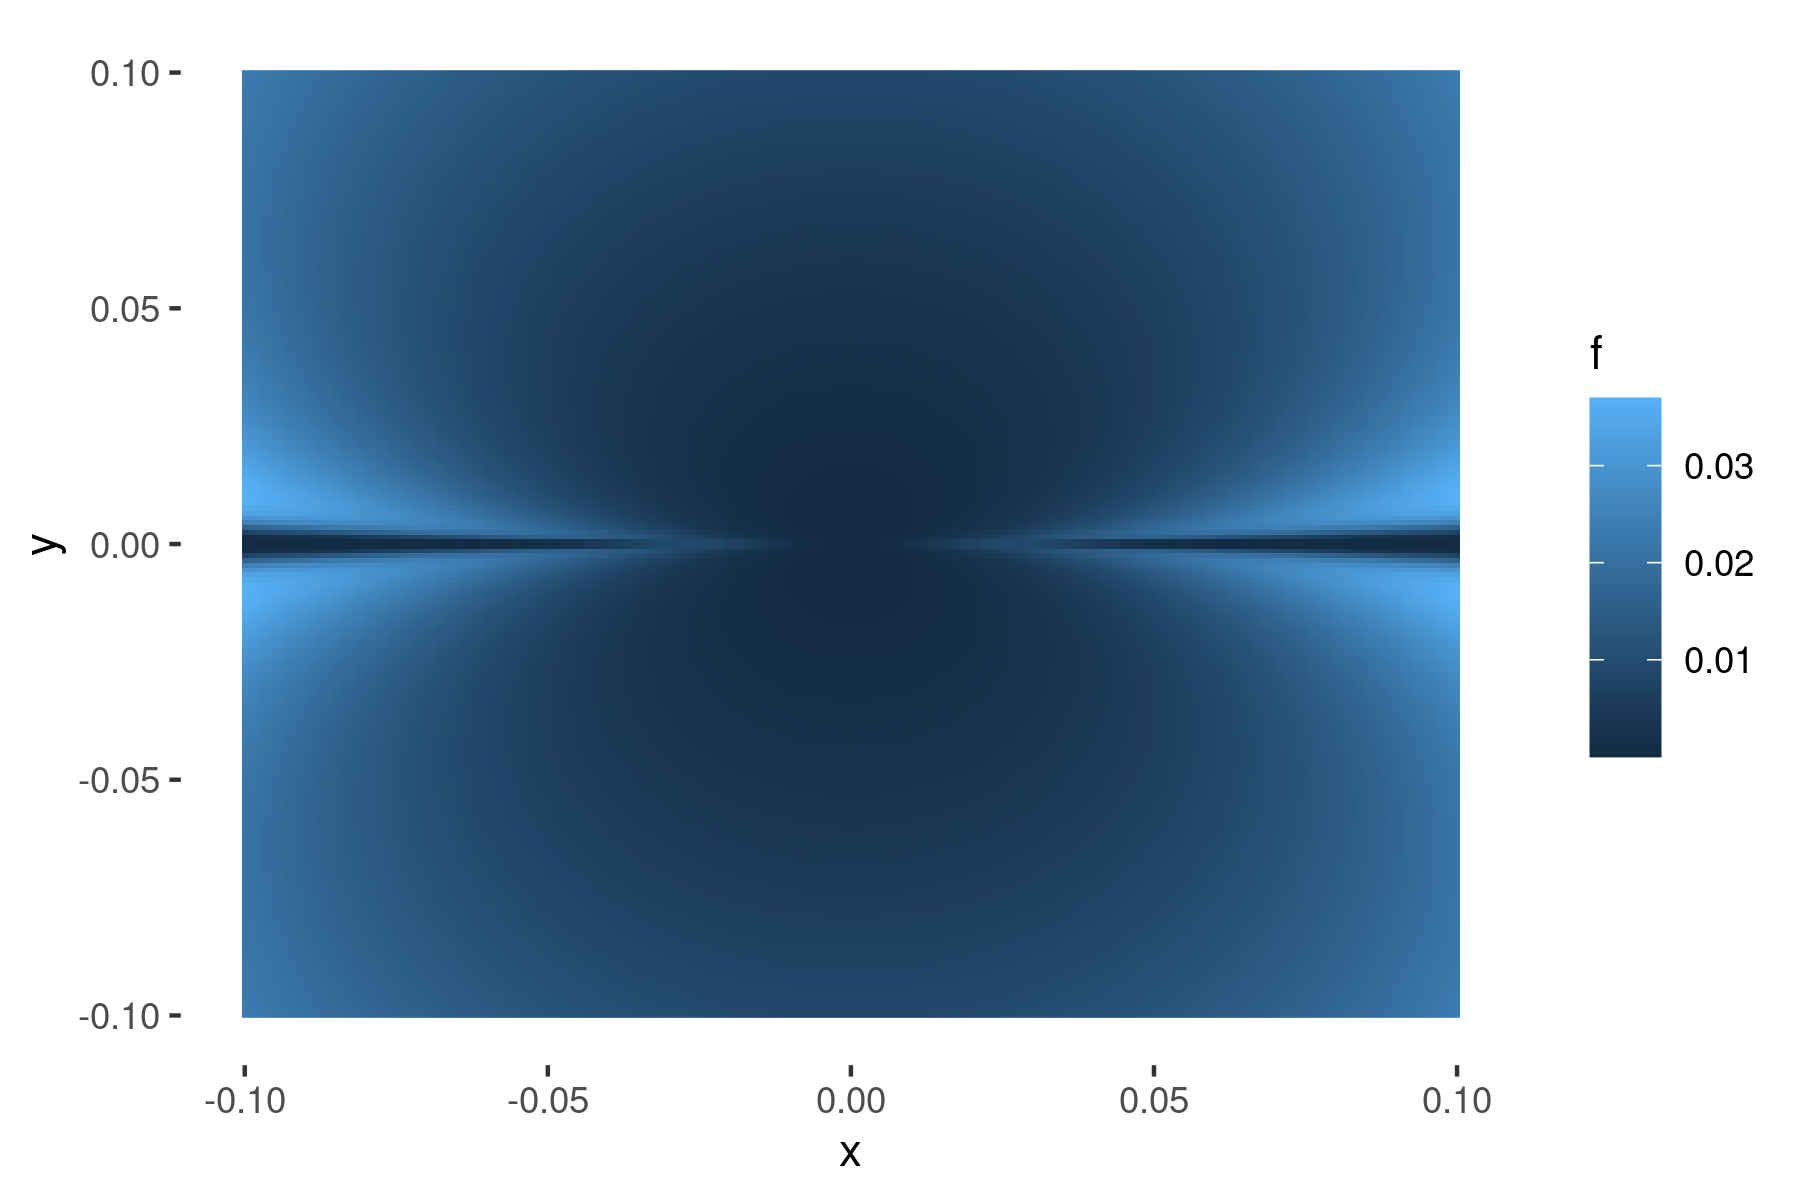
\includegraphics[width=0.980\linewidth,height=0.667\linewidth]{static_images/averbukh_example.png}
\caption{A plot of $f(x_1, x_2)$ from \exref{averbukh}.}\figlabel{averbukh_plot}
\centering
\end{figure}
%%%%%%%%%%%%%%%%%%%%%%%%%%%%%%%%%%%%%%%%%%%%%%%%%%%%%%%%%%%%%%%%%%%%%%%%%

































%%%%%%%%%%%%%%%%%%%%%%%%%%%%%%%%%%%%%%%%%%%%%%%%%%%%%%%%%%%%%%%%%%%%%%%%%
%%%%%%%%%%%%%%%%%%%%%%%%%%%%%%%%%%%%%%%%%%%%%%%%%%%%%%%%%%%%%%%%%%%%%%%%%
\begin{lem}\lemlabel{e_log_nonfrechet}

TODO: $\q$ should not be defined relative to $\lambda$.  And for
discontinuity we need
to require that there is a region such that
$\inf_\theta h(\theta) \q(\theta) p(\theta) > 0$.  Maybe it would be
better to just split this out into two different proofs?

Let $\lambda$ be continuous probability measure over $[0,1]$. Fix $1 \le p <
\infty$, and let $q = (1 - p^{-1})^{-1}$, from which $p^{-1} + q^{-1}=1$
follows.\footnote{Regrettably the standard choices of $p$ and $q$ for $\lp{p}$
spaces and their duals overlap with our notation for probability and variational
distributions, but there should be no ambiguity in context.}

Let $\q(\theta)$ be a density relative $\lambda$, and $h(\theta)$ a measurable
function such that $\int \abs{h(\theta)} \q(\theta) \lambda(d\theta) > 0$ and
$\int \abs{ \q(\theta) h(\theta)}^q \lambda(d\theta) < \infty$.

Let $\lp{\lambda,p}$ denote the space with the norm
$\norm{\phi}_{\lambda,p} := \left(\int \abs{\phi(\theta)}^p \lambda(d\theta)
\right)^{1/p}$.

Define $f: \lp{\lambda, p} \mapsto \mathbb{R}$ as follows:
%
\begin{align*}
%
f(\phi) :=
\begin{cases}
    %
    \expect{\q(\theta)}{h(\theta) \log \left(1 + \phi(\theta)\right)} &
    \textrm{when }0 < 1 + \phi(\theta)\textrm{ for all }\theta \\
    %
    0 & \textrm{otherwise}.
%
\end{cases}
%
\end{align*}
%
Then $f$ is discontinous at $\phiz$ and so not Fr{\'e}chet differentiable.
However $f$ has a directional derivative at $\phiz$ in every direction $\phi -
\phiz$.

\begin{proof}
%
Since $\int \abs{h(\theta)} \q(\theta) \lambda(d\theta) > 0$ we can choose a set
$S$ such that either $\inf_{\theta \in S} h(\theta) \q(\theta) \ge h_0$ or
$\inf_{\theta \in S} h(\theta) \q(\theta) \le -h_0$..........

Since $\lambda$ has a continuous component, for any sufficiently small $\epsilon >
0$, there exists a set $S_\epsilon$ with $\lambda(S_\epsilon) = \epsilon$. Since
$\int q(\theta) \lambda(d\theta) = 1$, we can find a set $S_\epsilon$ such that
$\int q(\theta) \lambda(d\theta) \ge \epsilon$ as well.\footnote{Were there no
such set, the measure under $\q$ of a partition of the domain into sets with
$\lambda$-measure no smaller than $\epsilon$ could not be $1$.}

For $\delta > 0$, let
%
\begin{align*}
%
\phi(\zeta; \epsilon, \delta) :=
\begin{cases}
    %
    \delta - 1      & \textrm{ for }\zeta\in S_\epsilon \\
    0      & \textrm{ for }\zeta\notin S_\epsilon.
    %
\end{cases}
%
\end{align*}
%
Then $\phi(\theta; \epsilon, \delta) \in \lp{\lambda,p}$ with $\norm{\phi(\cdot;
\epsilon, \delta)}_p = (\int_0^1 \phi(\theta)^p \lambda(d\theta)^{1/p}
=\epsilon^{1/p} (\delta - 1)$.  Furthermore,
%
\begin{align*}
%
\abs{f(\phi(\theta; \epsilon, \delta))} ={}&
    \expect{\q(\theta)}{\ind{\theta \in S_\epsilon}} \abs{\log(\delta)} \ge
    \epsilon \abs{\log(\delta)}.
%
\end{align*}
%,
Take $\delta(\epsilon) = \exp(-\epsilon)$.  Then, for any sequence $\epsilon_n
\rightarrow 0$,
%
\begin{align*}
%
\abs{f(\phi(\zeta; \epsilon_n, \delta(\epsilon_n))) - f(\phiz)} \ge{} 1
\mathtxt{and}
\norm{\phi(\cdot; \epsilon_n, \delta(\epsilon_n))}_p \rightarrow{} 0.
%
\end{align*}
%
So $f$ is discontinuous on an $\norm{\cdot}_p$ ball containing $\phiz$, and
cannot be Fr{\'e}chet differentiable.

We now show that the directional derivative exists in any direction.  First,
suppose that $\inf_{\theta} \phi(\zeta) = -\infty$.  Then $\inf_{\theta} t
\phi(\theta) = -\infty$ for any $t > 0$, so $f(t\theta) = 0$ for all $t$, and
$\lim_{t \rightarrow 0} (f(t \phi) - f(\phiz)) / t = \lim_{t \rightarrow 0} 0 =
0$.  Trivially, the directional derivative exists and is $0$ for $\phi$ that are
unbounded below.

If $-\infty < \inf_\theta \phi(\theta)$, then there exists a $t_0 > 0$ such that
$t_0 \phi(\theta)$ is strictly larger than $-1$.  Let us consider only $t <
t_0$. If we can apply the DCT, then
%
\begin{align*}
%
\fracat{\partial f(t \phi)}{\partial t}{t=0} ={}&
    \int \q(\theta) \fracat{\partial \log(1 + t \phi(\theta))}{\partial t}{t=0}
        \lambda(d\theta)
\\={}&
\int \q(\theta) \phi(\theta) \lambda(d\theta).
%
\end{align*}
%
The directional derivative in the direction $\phi - \phiz$ at $\phiz$ would thus
be given by $\expect{\q(\theta)}{\phi(\theta)}$.

We then need only to establish that we can apply the DCT. If $\sup_\theta
\phi(\theta) < \infty$ then we can apply the dominated convergence theorem with
a multiple of the constant function.  For the case $\sup_\theta \phi(\theta) =
\infty$, observe that
%
\begin{align*}
%
f(\phi) ={}&
    \int \q(\theta) \log(1 + \phi(\theta)) \ind{\phi(\theta) \le 0}
        \lambda(d\theta) + \\
    &\int \q(\theta) \log(1 + \phi(\theta)) \ind{\phi(\theta) > 0}
        \lambda(d\theta).
%
\end{align*}
%
The integrand $\log(1 + \phi(\zeta)) \ind{\zeta \le 0}$ of the first term
is bounded, so we can apply the DCT.  For the second term, the shape of
the logarithm gives
%
\begin{align*}
%
\q(\theta) \log(1 + t \phi(\theta)) \ind{t \phi(\theta) > 0}   \le{}&
    \q(\theta) (1 + t \phi(\theta)) \ind{t \phi(\theta) > 0}.%
\end{align*}
%
The preceding display is integrable for all finite $t$ whenever $\int \q(\theta)
\abs{\phi(\theta)} \lambda(d\theta) < \infty$. But this follows by Holder's
inequality, since
%
\begin{align*}
%
\int_0^1 \q(\theta) \abs{\phi(\theta)} \lambda(d \theta) \le{}&
    \left( \int \q(\theta)^q \lambda(d \theta) \right)^{1/q}
    \left( \int \abs{\phi(\theta)}^p \lambda(d \theta) \right)^{1/p}
\\={}&
    \left( \int \q(\theta)^q \lambda(d \theta) \right)^{1/q}
    \norm{\phi}_{\lambda,p}
\\\le{}&
    \infty.
%
\end{align*}
%
The result follows.
%
\end{proof}
%
\end{lem}
%%%%%%%%%%%%%%%%%%%%%%%%%%%%%%%%%%%%%%%%%%%%%%%%%%%%%%%%%%%%%%%%%%%%%%%%%





























It will be notationaly convenient in our discussion to treat the map $x \mapsto
\log(x)$ as simply discontinuous at $x = 0$, rather than undefined (or
complex-valued). Define the ``trimmed log'' function as

%%%%%%%%%%%%%%%%%%%%%%%%%%%%%%%%%%%%%%%%%%%%%%%%%%%%%%%%%%%%%%%%%%%%%%%%%
%%%%%%%%%%%%%%%%%%%%%%%%%%%%%%%%%%%%%%%%%%%%%%%%%%%%%%%%%%%%%%%%%%%%%%%%%
\begin{defn}
%
\begin{align*}
%
\logtrim(x) :=
\begin{cases}
    \log x  &\textrm{when }x > 0 \\
    0       &\textrm{when }x \le 0.
\end{cases}
%
\end{align*}
%
% In order for the directional derivative to exist in the direction of
% functions unbounded below, the value must be \log(1) = zero when undefined
%
% Otherwise, the when $x \le 0$ is simply a placeholder; for our purposes, it would
% ideally be some abstract number that is distant from all real numbers but zero
% distance to itself.  (Neither $0$ nor $\infty$ quite fit the bill.) Mostly we
% will require that $\logtrim(x)$ is discontinuous in a neighborhood of $0$.
%
\end{defn}
%%%%%%%%%%%%%%%%%%%%%%%%%%%%%%%%%%%%%%%%%%%%%%%%%%%%%%%%%%%%%%%%%%%%%%%%%


















% %
% \begin{align*}
% %
% \phi(\theta) ={}& \palt(\theta)^{1/p} - \pbase(\theta)^{1/p}
% \\={}&
% \pbase(\theta)^{1/p} \left(
%     \frac{\epsilon(1 - \delta)}{1 - \epsilon}
%         \ind{\theta \notin S_{\epsilon}} +
%     (\delta - 1) \ind{\theta \in S_{\epsilon}}
% \right) \Rightarrow \\
% %
% \norm{\phi}_{\lambda, p}^p ={}&
%     \int \pbase(\theta) \abs{\frac{\epsilon(1 - \delta)}{1 - \epsilon}}^p
%         \ind{\theta \notin S_{\epsilon}} \lambda(d\theta) +
%     \int \pbase(\theta) \abs{\delta - 1}^p \ind{\theta \in S_{\epsilon}}
%         \lambda(d\theta)
% \\={}&
%     (1-\epsilon)\abs{\frac{\epsilon(1 - \delta)}{1 - \epsilon}}^p +
%     \epsilon \abs{\delta - 1}^p
% \\={}&
% \epsilon \abs{\delta - 1}^p \left(1 + \frac{1}{(1 - \epsilon)^{p-1}} \right).
% %
% \end{align*}
% %
% And
% %
% \begin{align*}
% %
% \MoveEqLeft
%     \log\left(1 + \frac{\phi(\theta)}{\pbase(\theta)^{1/p}}\right)
% \\=&
%     \log\left(1 + \frac{\epsilon(1 - \delta)}{1 - \epsilon}\right)
%         \ind{\theta \notin S_{\epsilon}} +
%     \log\left(1 + (\delta - 1) \right) \ind{\theta \in S_{\epsilon}}.
% %
% \end{align*}
% %
% So
% %
% \begin{align*}
% %
% \MoveEqLeft
% \KL{\etaopt, \phi} - \KL{\etaopt, \phiz}
% \\={}&
%     \log\left(1 + \frac{\epsilon(1 - \delta)}{1 - \epsilon}\right)
%         \expect{\q(\theta \vert \etaopt)}{\ind{\theta \notin S_{\epsilon}}} +
%     \log\left( \delta \right)
%         \expect{\q(\theta \vert \etaopt)}{\ind{\theta \in S_{\epsilon}}}
%     \Rightarrow \\
% \MoveEqLeft
% \abs{\KL{\etaopt, \phi} - \KL{\etaopt, \phiz}}
% \\\ge{}&
% \epsilon \abs{\log \delta}
% - (1 - \epsilon) \log\left(1 + \frac{\epsilon(1 - \delta)}{1 - \epsilon}\right).
% %
% \end{align*}
% %
%
